\documentclass[a4paper,12pt]{article}
\usepackage[utf8]{inputenc}
\usepackage[T1]{fontenc}
\usepackage[ngerman]{babel}
\usepackage{lipsum}
\usepackage{titlesec} 
\usepackage[a4paper,left=2.5cm,right=2.5cm,top=2.5cm,bottom=2.5cm]{geometry}
\usepackage{setspace} 
\usepackage{parskip} 
\usepackage{graphicx} 
\usepackage[hidelinks]{hyperref}




\title{Verteilte Systeme - Blackout}
\author{Axel Walz, Tarek Bürner, David Langner}
\date{\today}


\titleformat{\section}[block]{\normalfont\Large\bfseries}{\thesection}{1em}{}
\titlespacing*{\section}{0pt}{\baselineskip}{\baselineskip}
\let\stdsection\section
\renewcommand\section{\newpage\stdsection}

\begin{document}

%\pagestyle{empty}
\onehalfspacing 

\maketitle

\newpage 
\tableofcontents
\newpage 
\pagestyle{plain}
\pagenumbering{arabic}

\section{Einführung Blackout}
In dem Buch "'Blackout – Morgen ist es zu spät"' von Marc Elsberg wird das fiktive Szenario eines europaweiten Stromausfalls beschrieben. Verursacht wird dieser durch die Manipulation der sogenannten Smart Meter. Dabei handelt es sich um intelligente Stromzähler, die Daten zum Verbrauch (und ggf. auch zur Erzeugung) an die Netzbetreiber übermitteln. Diese Daten ermöglichen es, Angebot und Nachfrage im Stromnetz effizienter zu regeln, was zu einer erhöhten Netzstabilität führt \cite{SmartMeter}. \\
Im Buch werden diese Smart Meter jedoch für einen Angriff auf das Stromnetz missbraucht, indem gefälschte Verbrauchsdaten an die Netzbetreiber gesendet werden. Diese simulierten Verbrauchsspitzen führen zu einem Abfall der Netzfrequenz. Sinkt die Netzfrequenz unter 49 Hz, werden Teile des Stromnetzes automatisch getrennt, um das System zu stabilisieren. Fällt die Frequenz weiter unter 47,5 Hz, trennen sich alle entsprechenden Netzsegmente vollständig vom Stromnetz, um größere Schäden zu vermeiden und anschließend die Stromversorgung neu aufzubauen \cite{Netzfrequenz}. Genau dies geschieht in "'Blackout"': Der Stromausfall beginnt in Norditalien. Aufgrund der engen Vernetzung der europäischen Stromnetze, die den Stromhandel und die Versorgungssicherheit gewährleisten sollen, weitet sich der Blackout von Italien auf Zentraleuropa und schließlich auf das gesamte europäische Stromnetz aus.\\
Zwar versuchen die betroffenen Länder immer wieder, die Stromversorgung neu aufzubauen, doch diese Bemühungen scheitern, da die Smart Meter kontinuierlich manipulierte Daten senden und somit eine stabile Frequenzregulierung verhindern. Dies führt zu einem nahezu zweiwöchigen Stromausfall in weiten Teilen Europas.\\
Das Buch "'Blackout"' verdeutlicht die Abhängigkeit moderner Gesellschaften von vernetzten Infrastrukturen und zeigt die Risiken auf, die durch Angriffe auf solche entstehen können. Gleichzeitig bietet es eine Grundlage, um die Rolle und Potenziale von Konzepten der Verteilten Systeme, zu analysieren. Diese können präventiv eingesetzt werden, um solche Szenarien zu verhindern oder deren Auswirkungen abzumildern. Im Folgenden werden drei zentrale Konzepte vernetzter Systeme – Event-Driven Architecture, Load Balancing und die Vermeidung von Single Points of Failure – näher beleuchtet, um die Brücke zwischen dem Buch und den Methoden verteilter Systeme zu schlagen.

\section{Event Driven Architecture}
\subsection{Grundlagen und Prinzipien}
Die Event Drive Architecture ist ein Architekturstil, der zu einer höheren Effizienz in Anwendungen führt. Dabei stehen Ereignisse im Vordergrund. Ereignisse beziehen sich auf die Veränderung eines Zustandes wie zum Beispiel die Veränderung einer gemessen Temperatur oder der Eingang eines HTTP Requests.
Als Ereignisgesteuert (event-driven) gilt ein System, wenn Aktionen innerhalb dieses Systems nicht einer festen Abfolge entsprechen sondern immer dynamisch eine Reaktion auf das Eintreffen eines Ereignisses ausgeführt werden.
Der zentrale Ablauf von ereignisgesteuerten Systemen besteht aus drei Schritten: Erkennen, Verarbeiten und Reagieren. \cite[S. 48f]{Bruns2010}

\textit{Erkennen}: In diesem Schritt wird ein Ereignis identifiziert, das eine Zustandsänderung signalisiert. Entscheidend hierfür ist, dass Ereignisse ohne Zeitverzögerung und somit unmittelbar nach ihrem Auftreten erkannt werden, um eine Reaktion mit geringer Verzögerung gewährleisten zu können.

\textit{Verarbeiten}: Das erkannte Ereignis wird während der Analyse abstrahiert, klassifiziert oder verworfen. Es wird darauf geachtet, dass bestimmte Beziehungen oder Abfolgen zwischen Ereignissen erkannt werden, die eine Aktion auslösen würde.

\textit{Reagieren}: Schließlich werden die vorbereiteten Aktionen ausgeführt, um auf das Ereignis zu reagieren und den neuen Zustand zu verarbeiten. Häufig vorkommende Reaktionen sind das Schicken von Warnmeldungen oder die Initiierung von Aktionen durch menschliche Benutzer. 

Um ein solches System zu realisieren muss während dem Erstellen der Softwarearchitektur darauf geachtet werden, dass es ohne eine zentrale Steuerung konzipiert wird. \cite[S. 50]{Bruns2010}

Da nicht jedes System, das Ereignisse beinhaltet direkt die Kriterien für ein Event Driven System erfüllt, gibt es zwei Eigenschaften, die ein ereignisgesteuerts System erfüllen muss. \newline
\textit{1. Verarbeitungsmodell:} \newline
Das Verarbeitungsmodell, das jedem ereignisgesteuerten Systemn zugrunde liegt, besteht aus drei ELementen: Ereignisquelle, Ereignissenke und Ereignisobjekt.
Ereignisquelle: Die Ereignisquelle, auch als Produzent bezeichnet, erkennt relevante Informationen und erzeugt Ereignisse, die als Nachrichten an einen Mediator gesendet werden. Der Mediator verteilt diese Nachrichten weiter, ohne dass die Ereignisquelle Details zur Verarbeitung oder zu den Empfängern kennen muss. Dadurch erreicht das System eine hohe Aktualität, da Ereignisse sofort nach ihrem Auftreten weitergeleitet werden.
Ereignissenke: Die Ereignissenke (Konsument) ist eine Komponente, die ein Ereignis empfängt und direkt darauf reagiert. Sobald ein Ereignis eintrifft, wird ein entsprechender Verarbeitungsvorgang ausgelöst.
Ereignisobjekt: Das Ereignisobjekt enthält nur Informationen über das Ereignis selbst, aber keine Details zur Reaktion darauf. Die Verarbeitung und die entsprechende Reaktion liegen vollständig bei der Ereignissenke. Dies verringert die Abhängigkeit zwischen Ereignisquelle und Ereignissenke was dazu führt, dass verschiedene Komponenten unabhängig voneinander auf dasselbe Ereignis reagieren können. \cite[S. 51f]{Bruns2010} \newline
Abbildung \ref{fig:Verarbeitungsmodell} veranschaulicht das Modell. 

\begin{figure}[h]
    \centering
    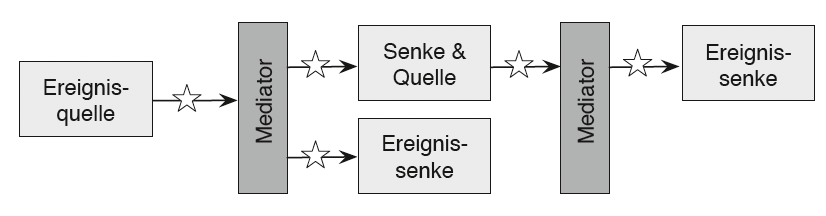
\includegraphics[width=0.8\textwidth]{images/Verarbeitungsmodell.png}
    \caption{Verarbeitungsmodell der Event Driven Architecture \cite[S. 52]{Bruns2010}}
    \label{fig:Verarbeitungsmodell}
\end{figure}

\textit{2. Kommunikationsmuster:} \newline
Das Kommunikationsmuster in einem ereignisgesteuerten System muss folgende Eigenschaften besitzen: Asynchronität, Publish/Subsribe-Interaktion und Push-Modus.
Asynchronität: Die Ereignisquelle sendet Nachrichten, ohne auf eine Antwort zu warten. Das bedeutet, dass Quelle und Empfänger unabhängig voneinander arbeiten können und nicht gleichzeitig aktiv sein müssen. Dadurch erhöht sich die Flexibilität und Effizienz der Kommunikation.
Publish/Subscribe-Interaktion: Die Ereignisquelle (“Publisher”) sendet Nachrichten an eine Middleware, und interessierte Empfänger (“Subscriber”) können diese Nachrichten abonnieren. Dies ermöglicht es mehreren Konsumenten, gleichzeitig auf dasselbe Ereignis zu reagieren.
Abbildung \ref{fig:PubSub} veranschaulicht das Modell.

\begin{figure}[h]
    \centering
    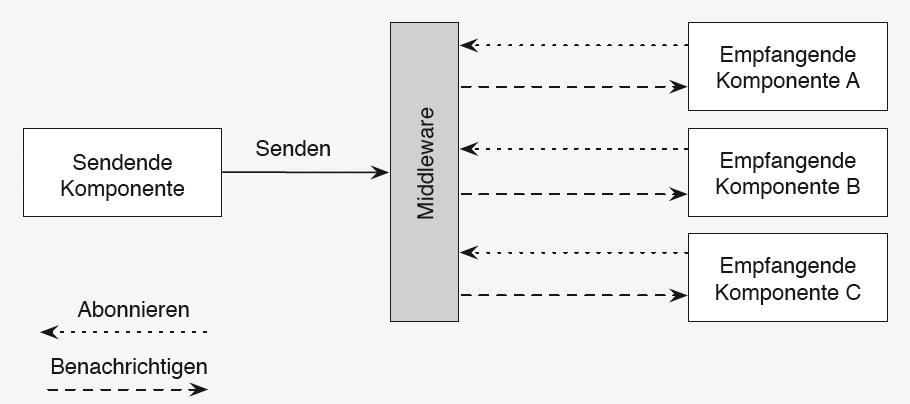
\includegraphics[width=0.8\textwidth]{images/Publish_Subscirbe.png}
    \caption{Publish/Subscirbe Interaktion \cite[S. 54]{Bruns2010}}
    \label{fig:PubSub}
\end{figure}
Push-Modus: Die Initiative zur Interaktion geht immer von der Ereignisquelle aus, die den Zeitpunkt des Nachrichtenaustauschs bestimmt. Dieses Push-basierte Modell ermöglicht eine hohe Entkopplung zwischen den Komponenten und fördert so die Skalierbarkeit und Interoperabilität des Systems. \cite [S. 53f]{Bruns2010}
\subsection{Beispielanwendungen in Bezug auf Blackout}
In Blackout wurden wie eingangs beschrieben Schadcodes über die intelligenten Stromzähler versendet, wodurch unregelmäßige Stromverbräuche simulliert wurden. Im Kontext der Event Driven Architecture, wäre hier ein Frühwarnsystem denkbar. Die Daten der Smart Meter würden hierbei als Ereignisquelle dienen. Um gezielt Angriffe erkennen zu können, muss hierbei überwachen, welcher Stromzähler zu welchen Zeitpunkten und in welchen Intervallen Daten sendet.\\
Anhand des übermittelten Ereignisses muss nun analysiert werden, ob Abweichungen vom normalen Betrieb zu identifizieren sind. Dafür könnten beispielsweise stark abweichende Verbrauchsmuster oder unerwartete Datenmuster als Indikatoren verwendet werden. Starke Lastspitzen oder besonders niedrige Werte wären eine Möglichkeit frühzeitig Angriffe zu erkennen.\\
Die Reaktion auf einen identifizierten Angriff sollte nun in unterschiedlichen Eskalationsstufen, durch die Ereignissenke erfolgen. Weißen bspw. nur einzelne Stromregler Unauffälligkeiten auf, reicht eine Warnmeldung an die zuständigen Instanzen und eine Überprüfung der Fehlerquelle. Sollten hingegen großflächig Unregelmäßigkeiten auftreten wodurch die Stabilität des Netzes gefährdet wird, müssen betroffene Bereiche automatisiert vom Netz getrennt werden um einen Blackout vermeiden zu können. Die Smart Meter verschicken die Daten zur Analyse asynchron, subscriben würden diejenigen Einrichtungen die zur Steuerung des Betroffenen Ausschnitts aus dem Stromnetz verantwortlich sind.\\
Eine EDA hätte also möglicherweise führen können, den Cyberangriff auf die Smart Meter als solchen zu identifizieren und den Europaweiten Blackout ggfs. auf lokale Blackouts reduzieren können.


\section{Load Balancing}
\subsection{Grundlagen und Funktionsweise}
In Abbildung \ref{fig:LoadBalancing} ist ein Beispielhaftes Modell des Load Balancing in der Cloud dargestellt. Load Balancing ist ein Verfahren, bei dem die Last auf mehrere Systeme verteilt wird, um die Leistung, Zuverlässigkeit und Verfügbarkeit eines Systems zu verbessern.
Ein Load Balancer erhält eine Anfrage von einem Clienten und entscheidet anhand Algorithmen, welcher Server oder Virtual Machine die Anfrage bearbeiten soll. 
Der \textit{Data Center Controller} verwaltet die Aufgaben, die an den Load Balancer übergeben werden. Dieser verwendet Algorithmen, um die Aufgaben an geeignete Virtual Machines zuzuweisen.

Benutzeranfragen werden weltweit zufällig eingereicht und müssen einer Virtual Machine zur Bearbeitung zugewiesen werden. Eine ungleichmäßige Auslastung der Virtual Machines kann die Servicequalität negativ beeinflussen. Ein \textit{Hypervisor} oder \textit{Virtual Machine Monitor} spielt dabei eine zentrale Rolle, da er die Erstellung und Verwaltung von Virtual Machines ermöglicht und Funktionen wie Multiplexing, Speicherung, Wiederaufnahme von zuvor gespeicherten Virtual Machines und Live-Migration zu einem anderen Host bereitstellt. \cite[S. 2]{LoadBalancing}

\begin{figure}[h]
    \centering
    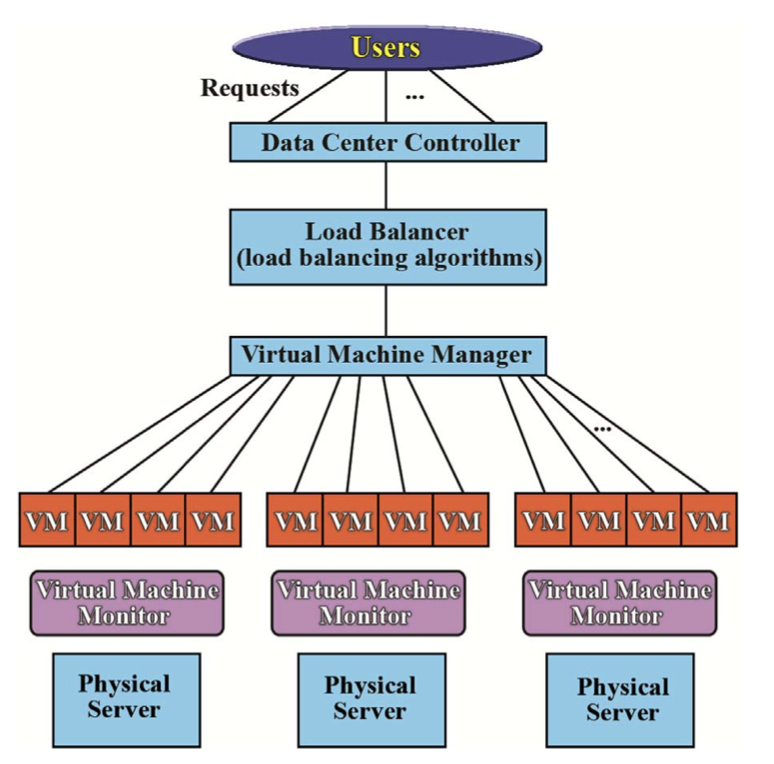
\includegraphics[width=0.5\textwidth]{images/Load_Balancing.png}
    \caption{Modell des Load Balancing \cite[S. 2]{LoadBalancing}}
    \label{fig:LoadBalancing}
\end{figure}

Es gibt verschiedene Arten von Load Balancing Algorithmen. Grob werden die Algorithmen aufgrund zwei verschiedener Faktoren eingeteilt: dem Zustand des Systems und der Person, die den Prozess initiert hat. 
Ersteres unterteilt sich weiter in statische und dynamische Algorithmen. Statische Algorithmen sind beispielsweise Round Robin, Min-Min oder Min Max Algorithmen. Diese setzen voraus, dass alle Systeminformationen im voraus bekannt sind. Ein Beispiel für einen dynamischen Algorithmus ist der Ant Colony Optimazation Algorithmus. Dynamische Algorithmen passen sich an die aktuelle Systemlast an und reagieren auf Änderungen in Echtzeit. 

Staische Algorithmen werden weiter in optimale und sub-optimale Algorithmen unterteilt. Optimal bedeutet, dass der Lastverteiler eine optimale Entscheidung basierend auf den vorhandenen Daten trifft. Sub-optimale Algorithmen treffen eine gute, aber nicht perfekte Entscheidung. Diese Algorithmen können heuristische oder approximative Methoden verwenden, um anpassungsfähige Entscheidungen zu treffen. Heuristische Methoden schätzen die Lösung basierend auf Erfahrungswerten, approximative Ansätze versuchen mathematisch nah an die optimale Lösung heranzukommen. 

Dynamische Algorithmen können weiter in verteilte und nicht-verteilte Klassen unterteilt werden. Bei den verteilten Algorithmen führen alle Knoten den Algorithmus aus und die Verteilung der Last ist zwischen den Knoten aufgeteilt. Zwischen den Knoten kann entweder eine kooperative oder nicht-kooperative Interaktion stattfinden. Bei der kooperativen Interaktion arbeiten die Knoten zusammen um das Ziel gemeinsam zu erreichen. Bei der nicht-kooperativen Interaktion verfolgt jeder Knoten sein eigenes lokales Ziel. Die nicht-verteilten dynamischen Algorithmen werden in zentralisierte und semi-verteilte Algorithmen unterteilt. Zentralisiert bedeutet, dass ein einzelner Knoten die Lastverteilung übernimmt. Semi-verteilt bedeutet, dass die Knoten in Gruppen organisiert sind und jeder Cluster einen zentralen Knoten hat, der für die Lastverteilung zuständig ist. 
\newline
Algorithmen, die von einer Person/einem Prozess initiert werden können entweder Sender-initiiert, Empfänger-initiiert oder symmetrisch sein.
Sender-initiiert bedeutet, dass Entscheidungen bei der Erstellung neuer Aufgaben getroffen werden. Empfänger-initiiert beudetet, dass Entscheidungen erfolgen, wenn Aufgaben abgeschlossen werden. Symmetrisch bedeutet, dass sowohl Sender als auch Empfänger Entscheidungen treffen können. \cite[S. 3]{LoadBalancing}

\subsection{Load Balancing zur Netzstabilität - Blackout}
Im Abschnitt EDA wurde bereits dargestellt, dass eine Analyse der Smart Meter-Daten möglicherweise zu einem abgeschwächten Stromausfall geführt hätte. Load Balancing bietet in Ergänzung mit EDA eine Möglichkeit, die Daten von den (potenziell) über 40 Millionen \cite{Haushalte} Smart Metern in Deutschland möglichst in Echtzeit zu analysieren. Damit würde Load Balancing ermöglichen, Abweichungen schnell zu erkennen und sofort darauf zu reagieren. So könnten in einem dynamischen, sich schnell verändernden Netz kritische Belastungen frühzeitig identifiziert und vermieden werden.\\
Ein solches System würde zudem ein prinzipiell stabileres Netz gewährleisten, indem die Stromnachfrage und das Angebot in Echtzeit optimal aufeinander abgestimmt werden. Dies ist besonders in Zeiten schwankender Energieerzeugung und -nachfrage wichtig, etwa bei der Integration erneuerbarer Energien. Durch Load Balancing könnte eine Überlastung von Netzabschnitten verhindert und die Energieeffizienz maximiert werden.\\
Darüber hinaus erhöht ein solches System die Resilienz des Stromnetzes gegen plötzliche Störungen. Im Falle eines gezielten Angriffs, etwa auf zentrale Steuerungseinheiten, oder einer technischen Fehlfunktion könnte das Load-Balancing-System automatisch alternative Lastverteilungen und Ausweichrouten schaffen. Diese Maßnahmen würden dazu beitragen, die Stromversorgung in kritischen Bereichen aufrechtzuerhalten und die Auswirkungen eines Blackouts zu minimieren. Besonders in einem Szenario wie im Buch \textit{Blackout} wäre ein solches Load-Balancing-System ein wichtiger Schutzmechanismus, um die Systemstabilität auch bei unerwarteten Ereignissen zu sichern.

\section{Single Point of Failure}

Ein SPOF ist eine Komponente eines Systems, deren Ausfall oder Defekt dazu führen kann, dass das gesamte System nicht mehr Funktioniert. In verteilten Systemen stellen SPOFs ein erhebliches Risiko für die Verfügbarkeit, Zuverlässigkeit und Sicherheit. Daher ist es wichtig SPOFs zu erkennen und zu beseitigen. 

\subsection{Ursachen und Risiken von SPOFs}
SPOFs entstehen häufig durch unzureichende Planung und Strukturierung. Eine häufige Ursache ist die Zentralisierung von Steuerungsinstanzen: Wenn Teilnehmer in einem verteilten System ohne eine zentrale Komponente wie eine Master-Node oder einen Hauptserver nicht eigenständig agieren können, wird diese Komponente zum SPOF. Fällt diese zentrale Stelle aus, führt dies zum Zusammenbruch des gesamten Systems \cite[S. 253f.]{Steen2006}.\\
Ein weiterer Faktor ist das Fehlen von Redundanz. Kritische Komponenten wie Datenbanken oder Kommunikationskanäle, die nicht durch Alternativen abgesichert sind, können bei einem Ausfall Systemfehler verursachen. Beispielsweise benötigen Stromnetze redundante Übertragungssysteme \cite[S. 61f.]{Jarass2009}. Auch Abhängigkeiten von einzelnen Technologien oder Dienstleistern erhöhen das Risiko. 


\subsection{Strategien zur Vermeidung von SPOFs}

Damit SPOFs vermieden werden können, müssen SPOFs zuerst identifiziert werden, um entsprechende Gegenmahnsamen vorzunehmen. Die Prozess der Identifikation von SPOFs beginnt bereits in der Planungsphase des Systems und wird beim Betrieb und jeder Änderung des Systems fortgeführt. Zur Identifikation gehören folgende Strategien:

\begin{itemize}
    \item \textbf{Architekturanalyse:} Die Systemarchitektur wird Analysiert um Abhängigkeiten zu erkennen, dabei helfen Architekturdiagramme SPOFs zu identifizieren. Dazu gehört auch die Identifikation von Abhängigkeiten von Drittanbietern, wie Cloud-Dienste.
    \item \textbf{Komponententests:} Der Ausfall einzelner Komponenten wird simuliert um dessen Auswirkung auf das Gesamtsystem zu bewerten.
    \item \textbf{Systemüberwachung:} Mithilfe von Monitoring-Daten werden häufig beanspruchte oder kritische Komponenten identifiziert. Des Weiteren wird das Netzwerk überwacht um Engpässe oder kritische Verbindungspunkte zu finden. 
\end{itemize}

Sobald die SPOF identifiziert sind, können sie durch folgende Strategien umgangen werden:

\begin{itemize}
    \item \textbf{Dezentralisierung:} Zentrale Steuerungsinstanzen werden vermieden, indem Funktionen auf mehrere Knoten verteilt werden, wie beispielsweise in Peer-to-Peer-Netzwerken.
    \item \textbf{Redundanz:} Kritische Komponenten werden mehrfach bereitgestellt, sodass ein Ausfall einer Komponente nicht zum Systemabsturz führt. Maßnahmen dafür sind die Datenreplikation, das Bereitstellen redundanter Server oder das Laufen von Paralleler Instanzen mit Load Balancing.
    \item \textbf{Failure Detectors und Failover-Mechanismen:} Failure Detectors erkennen Fehlerzustände um entsprechende Gegenmaßnahmen und Schutzmaßnahmen einzuleiten. wie zum Beispiel das Umschalten auf Backup-Systeme bei Ausfällen.
    \item \textbf{Systemseparierung:} Kritische Funktionen und Ressourcen werden in unabhängige, isolierte Einheiten aufgeteilt, sodass sich Probleme nicht auf das gesamte System ausbreiten können. Cloud-Services wie AWS setzen beispielsweise auf Instanzen in verschiedenen Verfügbarkeitskontrollen, sodass das Systemm selbst bei dem Ausfall eines Rechenzentrums aktiv bleibt.
\end{itemize}

\subsection{Angriffe auf Systeme ohne SPOF}
Systeme ohne SPOF bieten zwar einen besseren Schutz vor dem Ausfall einzelner Komponenten und gezielten Angriffen, sie sind jedoch nicht vollständig immun. Ein Angreifer könnte beispielsweise Failure Detectors manipulieren, um falsche Meldungen zu erzeugen. Dies kann dazu führen, dass korrekte Prozesse fälschlicherweise als ausgefallen markiert oder tatsächliche Fehler verschleiert werden. Auch "'eventually accurate"' Detektoren lassen sich so manipulieren, dass sie dauerhaft in einem Zustand der Unsicherheit bleiben. Es existieren jedoch Schutzmaßnahmen, die sicherstellen, dass trotz ungenauer Fehlererkennung keine Sicherheitsanforderungen verletzt werden. \cite{10.1145/1052796.1052806}

\subsection{SPOF in Blakout}
Das Buch \textit{Blackout} zeigt, wie essenziell ein funktionierendes Stromnetz für unsere moderne Gesellschaft ist. Ein Ausfall der Stromversorgung hätte gravierende Folgen: Die Lebensmittel- und Wasserversorgung kommt zum Erliegen, Krankenhäuser können nur noch für begrenzte Zeit ihren Betrieb aufrechterhalten – in vielen Fällen reicht die Notstromversorgung lediglich für 24 Stunden \cite{NotstromKrankenhaus}. Noch dramatischer gestaltet sich die Situation bei Kernkraftwerken, die oftmals lediglich eine Notstromversorgung von 10 Stunden gewährleisten können \cite[S. 11, Abschnitt 3.1.(9)]{NotstromAKWs}. Danach fallen die Kühlsysteme aus und es kann zu einem nuklearen Supergau kommen.
Obwohl das Buch ein fiktives Szenario darstellt, wird die Sicherheit und der Datenschutz von Smart Metern häufig kritisch hinterfragt. Kritiker bemängeln insbesondere die potenziellen Risiken für die Netzstabilität sowie die möglichen Angriffsflächen für Cyberangriffe \cite{SmartMeterBlackout}, \cite{SmartMeterSicherheit}.

\bibliographystyle{plain}
\bibliography{literatur}

\end{document}
